%--------------------
% Packages
% -------------------
\documentclass[11pt,english]{article}
\usepackage{amsfonts}
\usepackage[left=2.5cm,top=2cm,right=2.5cm,bottom=3cm,bindingoffset=0cm]{geometry}
\usepackage{amsmath, amsthm, amssymb}
\usepackage{tikz}
\usetikzlibrary{calc}
\usetikzlibrary{decorations.pathreplacing,calligraphy}
\usepackage{fancyhdr}
%\usepackage{currfile}
\usepackage{nicefrac}
\usepackage{cite}
\usepackage{graphicx}
\usepackage{caption}
\usepackage{longtable}
\usepackage{rotating}
\usepackage{lscape}
\usepackage{booktabs}
\usepackage{float}
\usepackage{placeins}
\usepackage{setspace}
\usepackage[font=itshape]{quoting}
\onehalfspacing
\usepackage{mathrsfs}
\usepackage{tcolorbox}
\usepackage{xcolor}
\usepackage{subcaption}
\usepackage{float}
\usepackage[multiple]{footmisc}
\usepackage[T1]{fontenc}
\usepackage[sc]{mathpazo}
\usepackage{listings}
\usepackage{longtable}
\definecolor{cmured}{RGB}{175,30,45}
\definecolor{macroblue}{RGB}{56,108,176}
\usepackage[format=plain,
            labelfont=bf,
            textfont=]{caption}
\usepackage[colorlinks=true,citecolor=macroblue,linkcolor=macroblue,urlcolor=macroblue]{hyperref}
\usepackage{varioref}
\usepackage{chngcntr}
\usepackage{datetime}

\definecolor{darkgreen}{RGB}{30,175,88}
\definecolor{darkblue}{RGB}{30,118,175}
\definecolor{maroon}{rgb}{0.66,0,0}
\definecolor{darkgreen}{rgb}{0,0.69,0}

%Counters
\newtheorem{theorem}{Theorem}[section] 
\newtheorem{proposition}{Proposition}
\newtheorem{lemma}{Lemma}
\newtheorem{corollary}{Corollary}
\newtheorem{assumption}{Assumption}
\newtheorem{axiom}{Axiom}
\newtheorem{case}{Case}
\newtheorem{claim}{Claim}
\newtheorem{condition}{Condition}
\newtheorem{definition}{Definition}
\newtheorem{example}{Example}
\newtheorem{notation}{Notation}
\newtheorem{remark}{Remark}


\hypersetup{ 	
pdfsubject = {},
pdftitle = {TidyTuesday Week 49},
pdfauthor = {Pranay Gundam},
linkcolor= macroblue
}


\title{\textbf{TidyTuesday Week 49}}
\author{Pranay Gundam}


%-----------------------
% Begin document
%-----------------------
\begin{document}

\maketitle

\tableofcontents

\section{Weekly Summary}


\section{Date: 2024-12-02}
\noindent \textbf{Series ID: CUUSX000SETA} 

\noindent This series is titled Consumer Price Index for All Urban Consumers: New and Used Motor Vehicles in Size Class B/C and has a frequency of Semiannual. The units are Index Dec 1997=100 and the seasonal adjustment is Not Seasonally Adjusted.The observation start date is 1998-01-01 and the observation end date is 2024-01-01.The popularity of this series is 1. \\ 

\noindent \textbf{Series ID: CUURX100SAGC} 

\noindent This series is titled Consumer Price Index for All Urban Consumers: Other Goods in Northeast - Size Class B/C and has a frequency of Monthly. The units are Index Dec 2009=100 and the seasonal adjustment is Not Seasonally Adjusted.The observation start date is 2009-12-01 and the observation end date is 2024-10-01.The popularity of this series is 2. \\ 

\subsection{Regression Tables and Plots}
\begin{center}
\begin{tabular}{lclc}
\toprule
\textbf{Dep. Variable:}            & value\_fred\_CUURX100SAGC & \textbf{  R-squared:         } &     0.750   \\
\textbf{Model:}                    &            OLS            & \textbf{  Adj. R-squared:    } &     0.741   \\
\textbf{Method:}                   &       Least Squares       & \textbf{  F-statistic:       } &     81.14   \\
\textbf{Date:}                     &      Mon, 02 Dec 2024     & \textbf{  Prob (F-statistic):} &  1.27e-09   \\
\textbf{Time:}                     &          15:39:20         & \textbf{  Log-Likelihood:    } &   -103.72   \\
\textbf{No. Observations:}         &               29          & \textbf{  AIC:               } &     211.4   \\
\textbf{Df Residuals:}             &               27          & \textbf{  BIC:               } &     214.2   \\
\textbf{Df Model:}                 &                1          & \textbf{                     } &             \\
\textbf{Covariance Type:}          &         nonrobust         & \textbf{                     } &             \\
\bottomrule
\end{tabular}
\begin{tabular}{lcccccc}
                                   & \textbf{coef} & \textbf{std err} & \textbf{t} & \textbf{P$> |$t$|$} & \textbf{[0.025} & \textbf{0.975]}  \\
\midrule
\textbf{const}                     &     -17.6595  &       15.608     &    -1.131  &         0.268        &      -49.685    &       14.366     \\
\textbf{value\_fred\_CUUSX000SETA} &       1.3099  &        0.145     &     9.008  &         0.000        &        1.012    &        1.608     \\
\bottomrule
\end{tabular}
\begin{tabular}{lclc}
\textbf{Omnibus:}       &  5.801 & \textbf{  Durbin-Watson:     } &    0.287  \\
\textbf{Prob(Omnibus):} &  0.055 & \textbf{  Jarque-Bera (JB):  } &    2.459  \\
\textbf{Skew:}          &  0.399 & \textbf{  Prob(JB):          } &    0.292  \\
\textbf{Kurtosis:}      &  1.817 & \textbf{  Cond. No.          } & 1.01e+03  \\
\bottomrule
\end{tabular}
%\caption{OLS Regression Results}
\end{center}

Notes: \newline
 [1] Standard Errors assume that the covariance matrix of the errors is correctly specified. \newline
 [2] The condition number is large, 1.01e+03. This might indicate that there are \newline
 strong multicollinearity or other numerical problems.

\begin{figure}
\centering
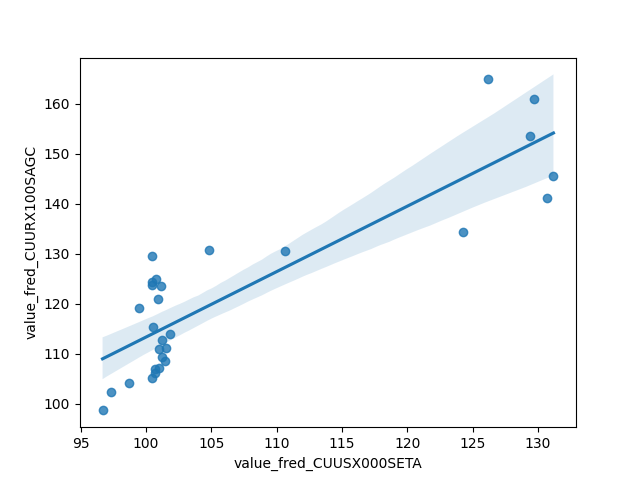
\includegraphics[scale = 0.9]{plots/plot_2024-12-02.png}
\caption{Regression Plot for 2024-12-02}
\end{figure}
\newpage

\section{Date: 2024-12-03}
\noindent \textbf{Series ID: M4241MM157NCEN} 

\noindent This series is titled Merchant Wholesalers, Except Manufacturers' Sales Branches and Offices: Nondurable Goods: Paper and Paper Products Sales and has a frequency of Monthly. The units are Percent and the seasonal adjustment is Not Seasonally Adjusted.The observation start date is 1992-02-01 and the observation end date is 2024-09-01.The popularity of this series is 1. \\ 

\noindent \textbf{Series ID: STFCFNQ} 

\noindent This series is titled Domestic Finance Companies; Capital, Surplus, and Undivided Profits and has a frequency of Quarterly. The units are Millions of Dollars and the seasonal adjustment is Not Seasonally Adjusted.The observation start date is 1984-01-01 and the observation end date is 2024-04-01.The popularity of this series is 1. \\ 

\subsection{Regression Tables and Plots}
\begin{center}
\begin{tabular}{lclc}
\toprule
\textbf{Dep. Variable:}              & value\_fred\_STFCFNQ & \textbf{  R-squared:         } &     0.010   \\
\textbf{Model:}                      &         OLS          & \textbf{  Adj. R-squared:    } &     0.002   \\
\textbf{Method:}                     &    Least Squares     & \textbf{  F-statistic:       } &     1.274   \\
\textbf{Date:}                       &   Tue, 03 Dec 2024   & \textbf{  Prob (F-statistic):} &    0.261    \\
\textbf{Time:}                       &       19:45:47       & \textbf{  Log-Likelihood:    } &   -1637.1   \\
\textbf{No. Observations:}           &           129        & \textbf{  AIC:               } &     3278.   \\
\textbf{Df Residuals:}               &           127        & \textbf{  BIC:               } &     3284.   \\
\textbf{Df Model:}                   &             1        & \textbf{                     } &             \\
\textbf{Covariance Type:}            &      nonrobust       & \textbf{                     } &             \\
\bottomrule
\end{tabular}
\begin{tabular}{lcccccc}
                                     & \textbf{coef} & \textbf{std err} & \textbf{t} & \textbf{P$> |$t$|$} & \textbf{[0.025} & \textbf{0.975]}  \\
\midrule
\textbf{const}                       &     2.02e+05  &     7045.089     &    28.672  &         0.000        &     1.88e+05    &     2.16e+05     \\
\textbf{value\_fred\_M4241MM157NCEN} &   -1300.4625  &     1152.056     &    -1.129  &         0.261        &    -3580.174    &      979.249     \\
\bottomrule
\end{tabular}
\begin{tabular}{lclc}
\textbf{Omnibus:}       &  0.166 & \textbf{  Durbin-Watson:     } &    0.052  \\
\textbf{Prob(Omnibus):} &  0.920 & \textbf{  Jarque-Bera (JB):  } &    0.264  \\
\textbf{Skew:}          &  0.080 & \textbf{  Prob(JB):          } &    0.876  \\
\textbf{Kurtosis:}      &  2.847 & \textbf{  Cond. No.          } &     6.18  \\
\bottomrule
\end{tabular}
%\caption{OLS Regression Results}
\end{center}

Notes: \newline
 [1] Standard Errors assume that the covariance matrix of the errors is correctly specified.

\begin{figure}
\centering
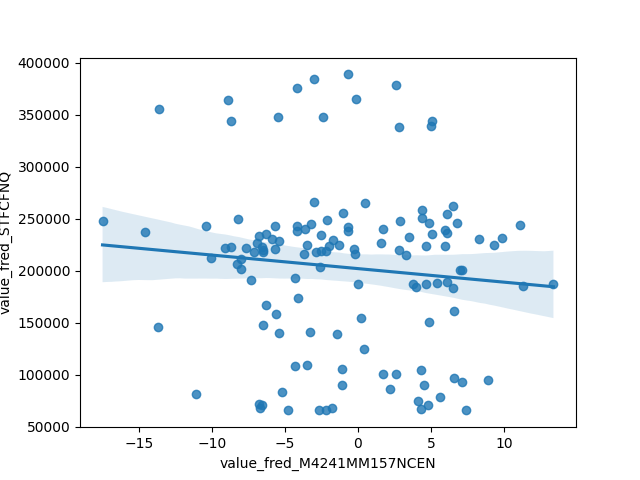
\includegraphics[scale = 0.9]{plots/plot_2024-12-03.png}
\caption{Regression Plot for 2024-12-03}
\end{figure}
\newpage

\section{Date: 2024-12-04}
\noindent \textbf{Series ID: CMTNPOP} 

\noindent This series is titled Resident Population in the Mountain Census Division and has a frequency of Annual. The units are Thousands of Persons and the seasonal adjustment is Not Seasonally Adjusted.The observation start date is 1900-01-01 and the observation end date is 2023-01-01.The popularity of this series is 2. \\ 

\noindent \textbf{Series ID: MNINEIPCMEPS} 

\noindent This series is titled Medical Services Expenditures per Capita by Disease: Mental Illness , MEPS Account Basis and has a frequency of Annual. The units are U.S. Dollars and the seasonal adjustment is Not Seasonally Adjusted.The observation start date is 2000-01-01 and the observation end date is 2021-01-01.The popularity of this series is 6. \\ 

\subsection{Regression Tables and Plots}
\begin{center}
\begin{tabular}{lclc}
\toprule
\textbf{Dep. Variable:}       & value\_fred\_MNINEIPCMEPS & \textbf{  R-squared:         } &     0.887   \\
\textbf{Model:}               &            OLS            & \textbf{  Adj. R-squared:    } &     0.882   \\
\textbf{Method:}              &       Least Squares       & \textbf{  F-statistic:       } &     157.6   \\
\textbf{Date:}                &      Wed, 04 Dec 2024     & \textbf{  Prob (F-statistic):} &  6.08e-11   \\
\textbf{Time:}                &          07:21:39         & \textbf{  Log-Likelihood:    } &   -112.09   \\
\textbf{No. Observations:}    &               22          & \textbf{  AIC:               } &     228.2   \\
\textbf{Df Residuals:}        &               20          & \textbf{  BIC:               } &     230.4   \\
\textbf{Df Model:}            &                1          & \textbf{                     } &             \\
\textbf{Covariance Type:}     &         nonrobust         & \textbf{                     } &             \\
\bottomrule
\end{tabular}
\begin{tabular}{lcccccc}
                              & \textbf{coef} & \textbf{std err} & \textbf{t} & \textbf{P$> |$t$|$} & \textbf{[0.025} & \textbf{0.975]}  \\
\midrule
\textbf{const}                &    -781.6050  &       91.548     &    -8.538  &         0.000        &     -972.570    &     -590.640     \\
\textbf{value\_fred\_CMTNPOP} &       0.0519  &        0.004     &    12.556  &         0.000        &        0.043    &        0.061     \\
\bottomrule
\end{tabular}
\begin{tabular}{lclc}
\textbf{Omnibus:}       &  4.125 & \textbf{  Durbin-Watson:     } &    0.471  \\
\textbf{Prob(Omnibus):} &  0.127 & \textbf{  Jarque-Bera (JB):  } &    2.380  \\
\textbf{Skew:}          &  0.761 & \textbf{  Prob(JB):          } &    0.304  \\
\textbf{Kurtosis:}      &  3.527 & \textbf{  Cond. No.          } & 2.30e+05  \\
\bottomrule
\end{tabular}
%\caption{OLS Regression Results}
\end{center}

Notes: \newline
 [1] Standard Errors assume that the covariance matrix of the errors is correctly specified. \newline
 [2] The condition number is large, 2.3e+05. This might indicate that there are \newline
 strong multicollinearity or other numerical problems.

\begin{figure}
\centering
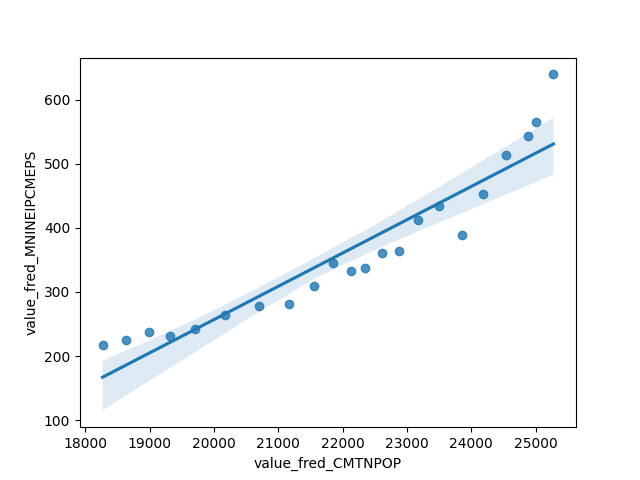
\includegraphics[scale = 0.9]{plots/plot_2024-12-04.png}
\caption{Regression Plot for 2024-12-04}
\end{figure}
\newpage

\include{tex_things/day_2024-12-05}
\include{tex_things/day_2024-12-06}
\include{tex_things/day_2024-12-07}
\section{Date: 2024-12-08}
\noindent \textbf{Series ID: BOPXSVN} 

\noindent This series is titled Exports of Services (DISCONTINUED) and has a frequency of Quarterly. The units are Billions of Dollars and the seasonal adjustment is Not Seasonally Adjusted.The observation start date is 1960-01-01 and the observation end date is 2014-01-01.The popularity of this series is 1. \\ 

\noindent \textbf{Series ID: FBTCMDODNS} 

\noindent This series is titled Farm Business; Credit Market Instruments; Liability (DISCONTINUED) and has a frequency of Quarterly, End of Period. The units are Billions of Dollars and the seasonal adjustment is Not Seasonally Adjusted.The observation start date is 1949-10-01 and the observation end date is 2015-01-01.The popularity of this series is 4. \\ 

\subsection{Regression Tables and Plots}
\begin{center}
\begin{tabular}{lclc}
\toprule
\textbf{Dep. Variable:}       & value\_fred\_FBTCMDODNS & \textbf{  R-squared:         } &     0.692   \\
\textbf{Model:}               &           OLS           & \textbf{  Adj. R-squared:    } &     0.690   \\
\textbf{Method:}              &      Least Squares      & \textbf{  F-statistic:       } &     482.0   \\
\textbf{Date:}                &     Sun, 08 Dec 2024    & \textbf{  Prob (F-statistic):} &  8.04e-57   \\
\textbf{Time:}                &         11:53:47        & \textbf{  Log-Likelihood:    } &   -1098.2   \\
\textbf{No. Observations:}    &             217         & \textbf{  AIC:               } &     2200.   \\
\textbf{Df Residuals:}        &             215         & \textbf{  BIC:               } &     2207.   \\
\textbf{Df Model:}            &               1         & \textbf{                     } &             \\
\textbf{Covariance Type:}     &        nonrobust        & \textbf{                     } &             \\
\bottomrule
\end{tabular}
\begin{tabular}{lcccccc}
                              & \textbf{coef} & \textbf{std err} & \textbf{t} & \textbf{P$> |$t$|$} & \textbf{[0.025} & \textbf{0.975]}  \\
\midrule
\textbf{const}                &      76.1363  &        3.548     &    21.456  &         0.000        &       69.142    &       83.131     \\
\textbf{value\_fred\_BOPXSVN} &       1.1835  &        0.054     &    21.954  &         0.000        &        1.077    &        1.290     \\
\bottomrule
\end{tabular}
\begin{tabular}{lclc}
\textbf{Omnibus:}       & 26.816 & \textbf{  Durbin-Watson:     } &    0.013  \\
\textbf{Prob(Omnibus):} &  0.000 & \textbf{  Jarque-Bera (JB):  } &   32.716  \\
\textbf{Skew:}          &  0.918 & \textbf{  Prob(JB):          } & 7.87e-08  \\
\textbf{Kurtosis:}      &  3.500 & \textbf{  Cond. No.          } &     89.7  \\
\bottomrule
\end{tabular}
%\caption{OLS Regression Results}
\end{center}

Notes: \newline
 [1] Standard Errors assume that the covariance matrix of the errors is correctly specified.

\begin{figure}
\centering
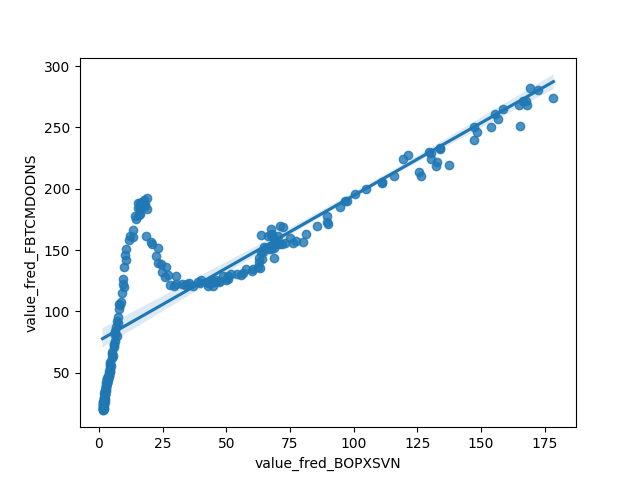
\includegraphics[scale = 0.9]{plots/plot_2024-12-08.png}
\caption{Regression Plot for 2024-12-08}
\end{figure}
\newpage


\end{document}
